% Autor: Simon May
% Datum: 2017-10-05
% Diese Datei bietet ein minimalistisches Grundgerüst für ein LaTeX-Dokument,
% z.B. für die Bearbeitung der Aufgaben.
\documentclass[
	% Papierformat
	a4paper,
	% Schriftgröße (beliebige Größen mit „fontsize=Xpt“)
	12pt,
	% Schreibt die Papiergröße korrekt ins Ausgabedokument
	pagesize,
	% Sprache für z.B. Babel
	ngerman
]{scrartcl}

% Achtung: Die Reihenfolge der Pakete kann (leider) wichtig sein!
% Insbesondere sollten (so wie hier) babel, fontenc und inputenc (in dieser
% Reihenfolge) als Erstes und hyperref und cleveref (Reihenfolge auch hier
% beachten) als Letztes geladen werden!

% Silbentrennung etc.; Sprache wird durch Option bei \documentclass festgelegt
\usepackage{babel}
% Verwendung der Zeichentabelle T1 (Sonderzeichen etc.)
\usepackage[T1]{fontenc}
% Legt die Zeichenkodierung der Eingabedatei fest, z.B. UTF-8
\usepackage[utf8]{inputenc}
% Schriftart
\usepackage{lmodern}
% Zusätzliche Sonderzeichen
\usepackage{textcomp}

% Mathepaket (intlimits: Grenzen über/unter Integralzeichen)
\usepackage[intlimits]{amsmath}
% Ermöglicht die Nutzung von \SI{Zahl}{Einheit} u.a.
\usepackage{siunitx}
% Zum flexiblen Einbinden von Grafiken (\includegraphics)
\usepackage{graphicx}
% Abbildungen im Fließtext
\usepackage{wrapfig}
% Abbildungen nebeneinander (subfigure, subtable)
\usepackage{subcaption}
% Funktionen für Anführungszeichen
\usepackage{csquotes}
% Zitieren, Bibliographie
\usepackage{biblatex}

% Verlinkt Textstellen im PDF-Dokument
\usepackage[unicode]{hyperref}
% "Schlaue" Referenzen (nach hyperref laden!)
\usepackage{cleveref}

% siunitx: Deutsche Ausgabe, Messfehler getrennt mit ± ausgeben
\sisetup{
	locale=DE,
	separate-uncertainty
}

\begin{document}
\begin{titlepage}
	\centering
	{\scshape\LARGE Versuchsbericht zu \par}
	\vspace{1cm}
	{\scshape\huge MP3 - Versuch zur Al-Rekristallisation \par}
	\vspace{2.5cm}
	{\LARGE Gruppe D-01\par}
	\vspace{0.5cm}
	{\large Nils Kulawiak (E-Mail: n\_kula01@wwu.de) \par}
	{\large Oliver Brune (E-Mail: o\_brun02@wwu.de) \par}
	{\large Anthony Pietz (E-Mail: a\_piet09@wwu.de) \par}
	\vfill
	durchgeführt am 12.11.2018\par
	
	\vfill
	betreut von Lena Frommeyer\par
	\vfill
	{\large \today\par}
\end{titlepage}

\tableofcontents
		
\newpage
\section{Kurzfassung}
In diesem Versuch werden die Auswirkungen von hohen Temperaturen auf die Verformung, Härte und Korngröße von Aluminium untersucht. 
Dazu werden zuerst Aluminiumproben mithilfe einer Walze um unterschiedliche Verformungsgrade verformt 
und anschließend bei unterschiedlichen Temperaturen in Öfen erhitzt.
Im ersten Versuchsteil wird der Einfluss der Temperatur, mit der die Proben erhitzt werden, auf den Ausheilungsprozess untersucht.
Dazu werden zuerst acht $80\%$-verformte Proben bei unterschiedlichen Temperaturen fünf Minuten erhitzt. 
Anschließend wird die Vickers-Härte der Proben bestimmt, über die Rückschlüsse auf den Grad der Verformung bzw. Grad der Ausheilung gezogen werden können. 
Es zeigt sich, dass die Proben bei höheren Temperaturen schneller ausheilen, da die Rekristallisation hier schneller abläuft.
Im zweiten Teil wurde der Verformungsgrad auf die Anzahl der Körner aufgetragen. Anhand der Graphen konnten drei Bereiche beobachtet werden. Im ersten Bereich hat die Anzahl der Körner mit steigender Verformung abgenommen. Im zweiten Teil hat die Anzahl dann exponentiell zugenommen und im dritten Teil konvergierte die Anzahl an Körnern bei steigendem Verformungsgrad. Der zeite Teil dieser Beobachtung wurde über ein Auswertungsprogramm geplottet. Die anderen beiden Bereiche wurden in der Diskussion erläutert.


\section{Härte von Aluminium}
\subsection{Methoden und Durchführung}
Zuerst mussten alle verwendeten Proben um einen bestimmten Grad verformt werden. Dafür wurden sie mit einer Walze dünner gewalzt. Um einen bestimmten Verformungsgrad zu erreichen, wurde zuerst mit \cref{eq:ver} die benötigte Dicke der Probe berechnet. Die Probe wurde anschließend auf die berechnete Dicke gewalzt.

\begin{equation}
V = \frac{d_0-d}{d_0} \cdot 100
\label{eq:ver}
\end{equation}

Anschließend wurden die Proben in verschiedene Öfen gegeben. Einerseits wurden sieben Proben, die alle auf einen Verformungsgrad von $80\%$ verformt wurden, auf sieben Öfen mit verschiedenen Temperaturen verteilt, in denen sie jeweils fünf Minuten erhitzt wurden. Eine Probe wurde nicht erhitzt, sondern bei Raumtemperatur gelassen. Andererseits wurden acht Proben mit verschiedenen Verformungsgraden in einem Ofen mit $550\%$ für eine Stunde erhitzt. Alle Proben wurden nach der Zeit im Ofen in kaltem Wasser schnell auf Raumtemperatur abgekühlt, um die Ergebnisse durch einen langsamen Abkühlprozess nicht zu verfälschen. Die beiden Probenpakete wurden anschließend mit unterschiedlichen Verfahren weiter untersucht.

Bei den Proben mit gleichem Verformungsgrad, aber unterschiedlicher Heiztemperatur, wurde im weiteren die Vickers-Härte gemessen. Hierbei wird ein Diamant in Form einer Pyramide mit fester Kraft für fünf Sekunden in die Probe gedrückt. Die Vickers-Härte wird nun aus der Eindringtiefe der Pyramide und der Kraft, mit der auf die Probe gedrückt wird, berechnet. Die Eindringtiefe wird aus der Breite des Abdrucks der Pyramide bestimmt. Diese Rechnung führt der verwendete Vickers-Härteprüfer automatisch aus. Da die Härte eines Stoffs bei starker Verformung steigt, ist die Vickers Härte in diesem Versuch ein Maß dafür, wie stark die Kristallbaufehler der Proben nach der Zeit im Ofen ausgeheilt sind. Eine höhere Vickers-Härte bedeutet daher starke Verformung, also viele Kristallbaufehler, eine niedrige Vickers-Härte steht für schwache Verformung, also eine stark ausgeheilte Probe. Für jede Probe wurden drei Werte aufgenommen.

\subsection{Auswertung}

In \cref{vickers} wurde die Vickers-Härte gegen die Temperatur aufgetragen. Von Raumtemperatur bis etwa $\SI{140}{\degreeCelsius}$ ist die Vickers-Härte nahezu konstant bei $44-45$HV. Zwischen $\SI{190}{\degreeCelsius}$ und $\SI{350}{\degreeCelsius}$ sinkt die Härte, bis sie einen Wert von $22$ HV erreicht. Für höhere Temperaturen bleibt die Vickers-Härte konstant auf diesem Wert.

\begin{figure}[h]
	\centering
	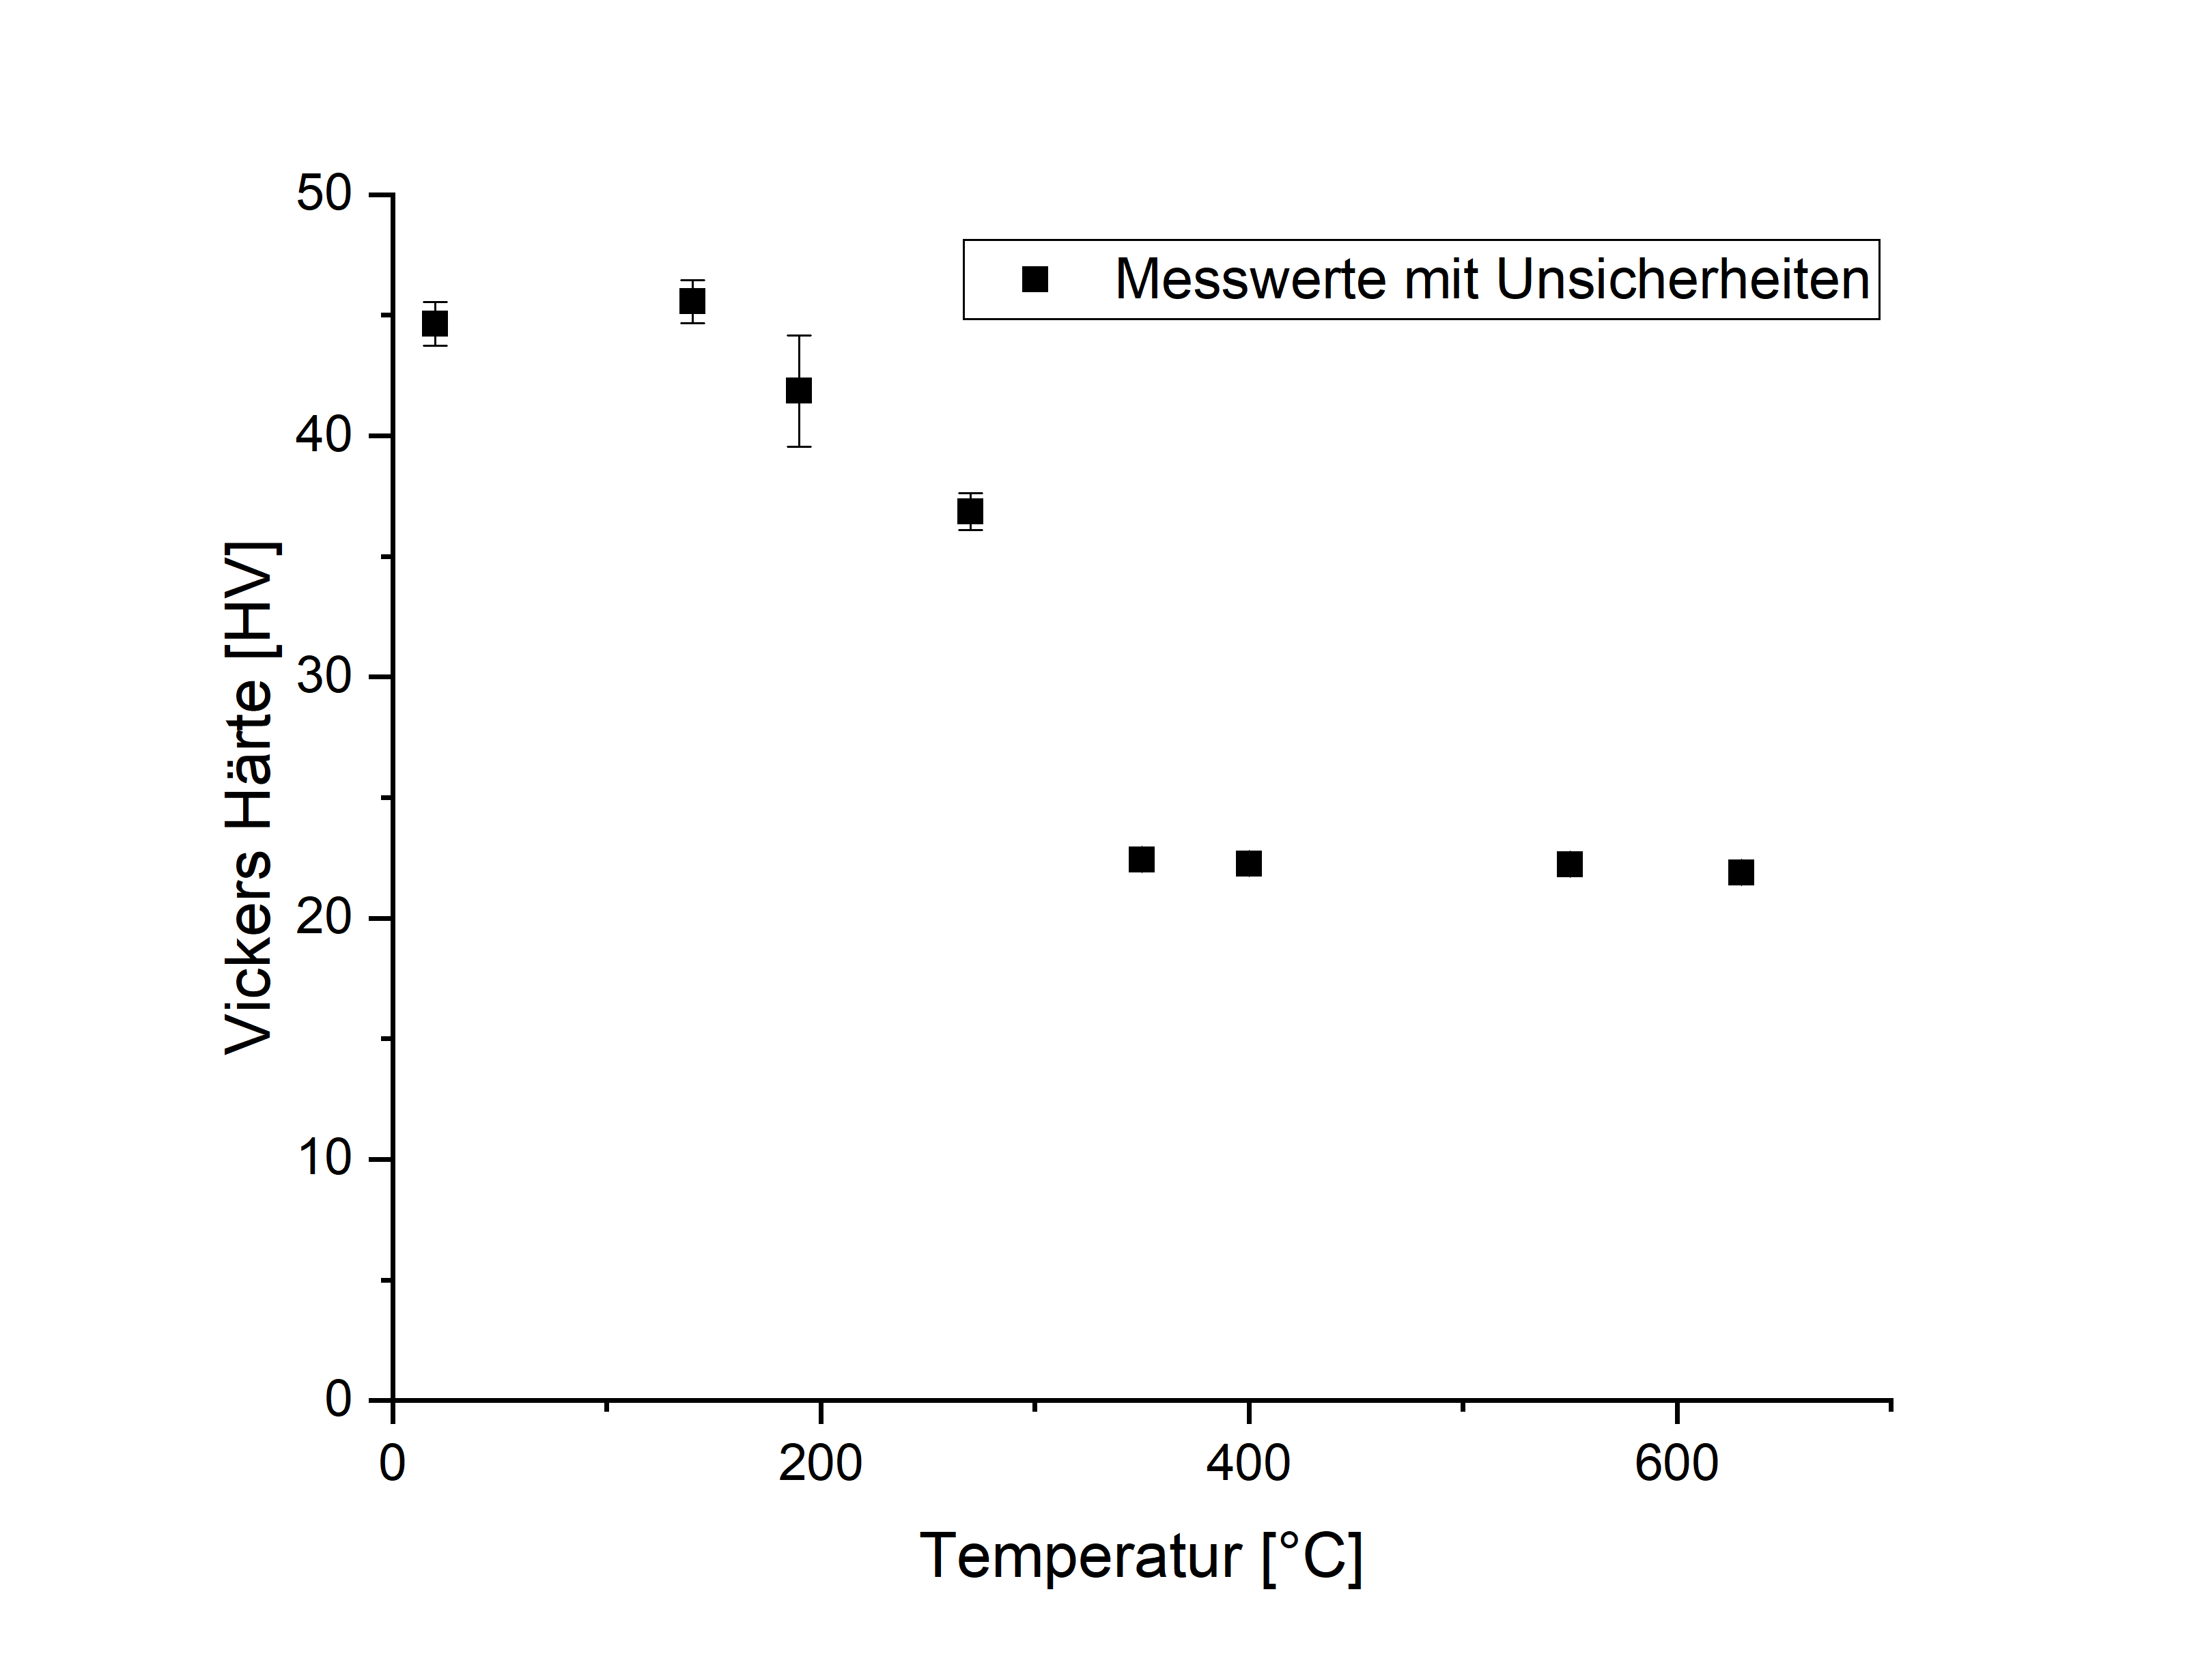
\includegraphics[scale=0.6]{vickers.png}
	\caption{Die Vickers-Härte aufgetragen gegen die Temperatur, bei der die Probe vorher für fünf Minuten im Ofen erhitzt wurde.}
	\label{vickers}
\end{figure}

Die Unsicherheit ergibt sich aus der Standardabweichung um den Mittelwert, der aus den drei Messwerten pro Probe berechnet wird. Sie ist nur für die Probe bei $\SI{190}{\degreeCelsius}$ mit $\pm2,31$ etwas größer, ansonsten ist sie vernachlässigbar klein.

\begin{figure}[h]
	\centering
	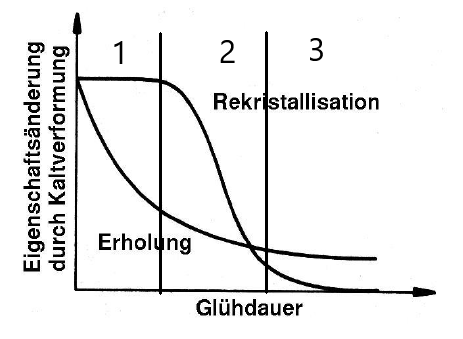
\includegraphics[scale=1]{grafik1.png}
	\caption{Zeitlicher Ablauf der Erholung und Rekristallisation (schematisch)}
	\label{grafik}
\end{figure}

Bei der Ausheilung von Kristallbaufehlern spielen zwei Prozesse eine Rolle: Erholung und Rekristallisation. Die Rekristallisation ist stark von der Temperatur abhängig. Die Zeit, die ein Kristall zur Rekristallisation benötigt, sinkt exponentiell bei höherer Temperatur. Eine Rolle spielt außerdem die unterschiedliche Geschwindigkeit, mit der beide Prozesse ablaufen. Die Kinetik beider Prozesse ist in \cref{grafik} dargestellt, außerdem sind drei Phasen der Rekristallisation eingezeichnet. Die Erholungsgeschwindigkeit ist zu Beginn am größten, sinkt aber über längere Zeit immer weiter ab.Bei der Rekristallisation dagegen müssen sich zuerst neue Körner bilden. In diesem Zeitraum bleibt die Verformung konstant (Phase 1). Nach einiger Zeit fangen die Körner stärker an zu wachsen, hier werden sehr schnell viele Kristallbaufehler berichtigt (Phase 2). Wenn die Körner so groß geworden sind, dass sich die Korngrenzen berühren, endet der Prozess, die Verformung bleibt konstant (Phase 3). Über diese beiden Zusammenhänge lässt sich der Verlauf der Messwerte in \cref{vickers} erklären.

Bei den ersten beiden Temperaturen ist die Rekristallisationszeit noch sehr groß, die Keime bilden sich so langsam, dass sich die Rekristallisation nach den fünf Minuten im Ofen noch in Phase 1 befindet. Die Proben von $\SI{190}{\degreeCelsius}$ bis $\SI{350}{\degreeCelsius}$ befinden sich nach der Erhitzung in Phase 2, es haben sich bereits größere Körner gebildet, diese sind allerdings noch nicht ausgewachsen. Die restlichen Proben sind nach fünf Minuten im Ofen bereits vollständig rekristallisiert, sie befinden sich in Phase 3. Die Rekristallisationszeit ist hier kleiner als fünf Minuten.

Die Vickers-Härte, und damit auch die Ausheilung der Proben, ist in diesem Versuch unabhängig von der Erholung und lässt sich vollständig durch Rekristallisation erklären. Das liegt daran, dass die Erholung am Anfang stark ist und mit der Zeit schwächer wird und nicht so stark von der Temperatur abhängt wie die Rekristallisation, sondern auch bei Raumtemperatur stattfindet. Da zwischen der Verformung der Proben und der Messung der Vickers-Härte mehrere Stunden lagen, konnten sich die Proben in dieser Zeit bereits sehr stark erholen. Da die Erholung nach längerer Zeit sowieso kaum noch Auswirkung auf die Ausheilung hat, spielt sie für den Verlauf der Messwerte in \cref{vickers} keine Rolle.

\section{Korngröße von Aluminium}
\subsection{Methoden}
In diesem Teil des Berichtes wird beschrieben, wie die technischen Apparaturen aussahen, um die Korngröße in Abhängigkeit vom Verformungsgrad (V) zu messen. Dazu wurden acht Aluminium-Proben durch eine Kaltwalze verformt. Zuerst wurde die Anfangsdicke der Aluminiumplatten ($d_0$) mit einer Mikrometerschraube ausgemessen. Dann wurden die Platten durch die Kaltwalze verformt. Im Nachhinein wurde dann die Verformte Dicke der Aluminiumplatten (d) gemessen. Über \cref{eq:ver} konnte dann der Verformungsgrad errechnet werden.

Die Verformung betrug 0\%, 2,5\%, 5\%, 10\%, 20\%, 30\%, 40\% und 50\%.
Die einzelnen Proben wurden dann eine Stunde lang auf 550°C erhitzt. Dadurch wurde der Prozess der Rekristallisation beschleunigt, d.h. der Prozess der Körnerbildung beginnt. Nach einer Stunde wurden die Proben durch ein Kältebad abgekühlt, sodass die räumliche Struktur des Aluminiums einfriert und beobachtet werden kann. Dafür wurden die Aluminiumplatten chemisch behandelt, sodass eine Kornstruktur sichtbar wurde. Nach der Behandlung konnte man durch eine Linearanalyse die Anzahl der Körner pro Zentimeter bestimmen.

\subsection{Auswertung}
Durch die Linearanalyse konnte man die Anzahl der Körner bei verschiedenen Verformungsgraden bestimmen. Dazu wurde eine Strecke quer über das Aluminiumplättchen gezogen und gezählt, wie viele Körner sich auf der Linie befinden. Dies ist ein Mittelwert für die Anzahl der Körner pro Zentimeter. 
Dieses Mittel wurde über den Verformungsgrad aufgetragen.
Daraus ergab sich \cref{A1}.
\begin{figure}[h!]
    \centering
    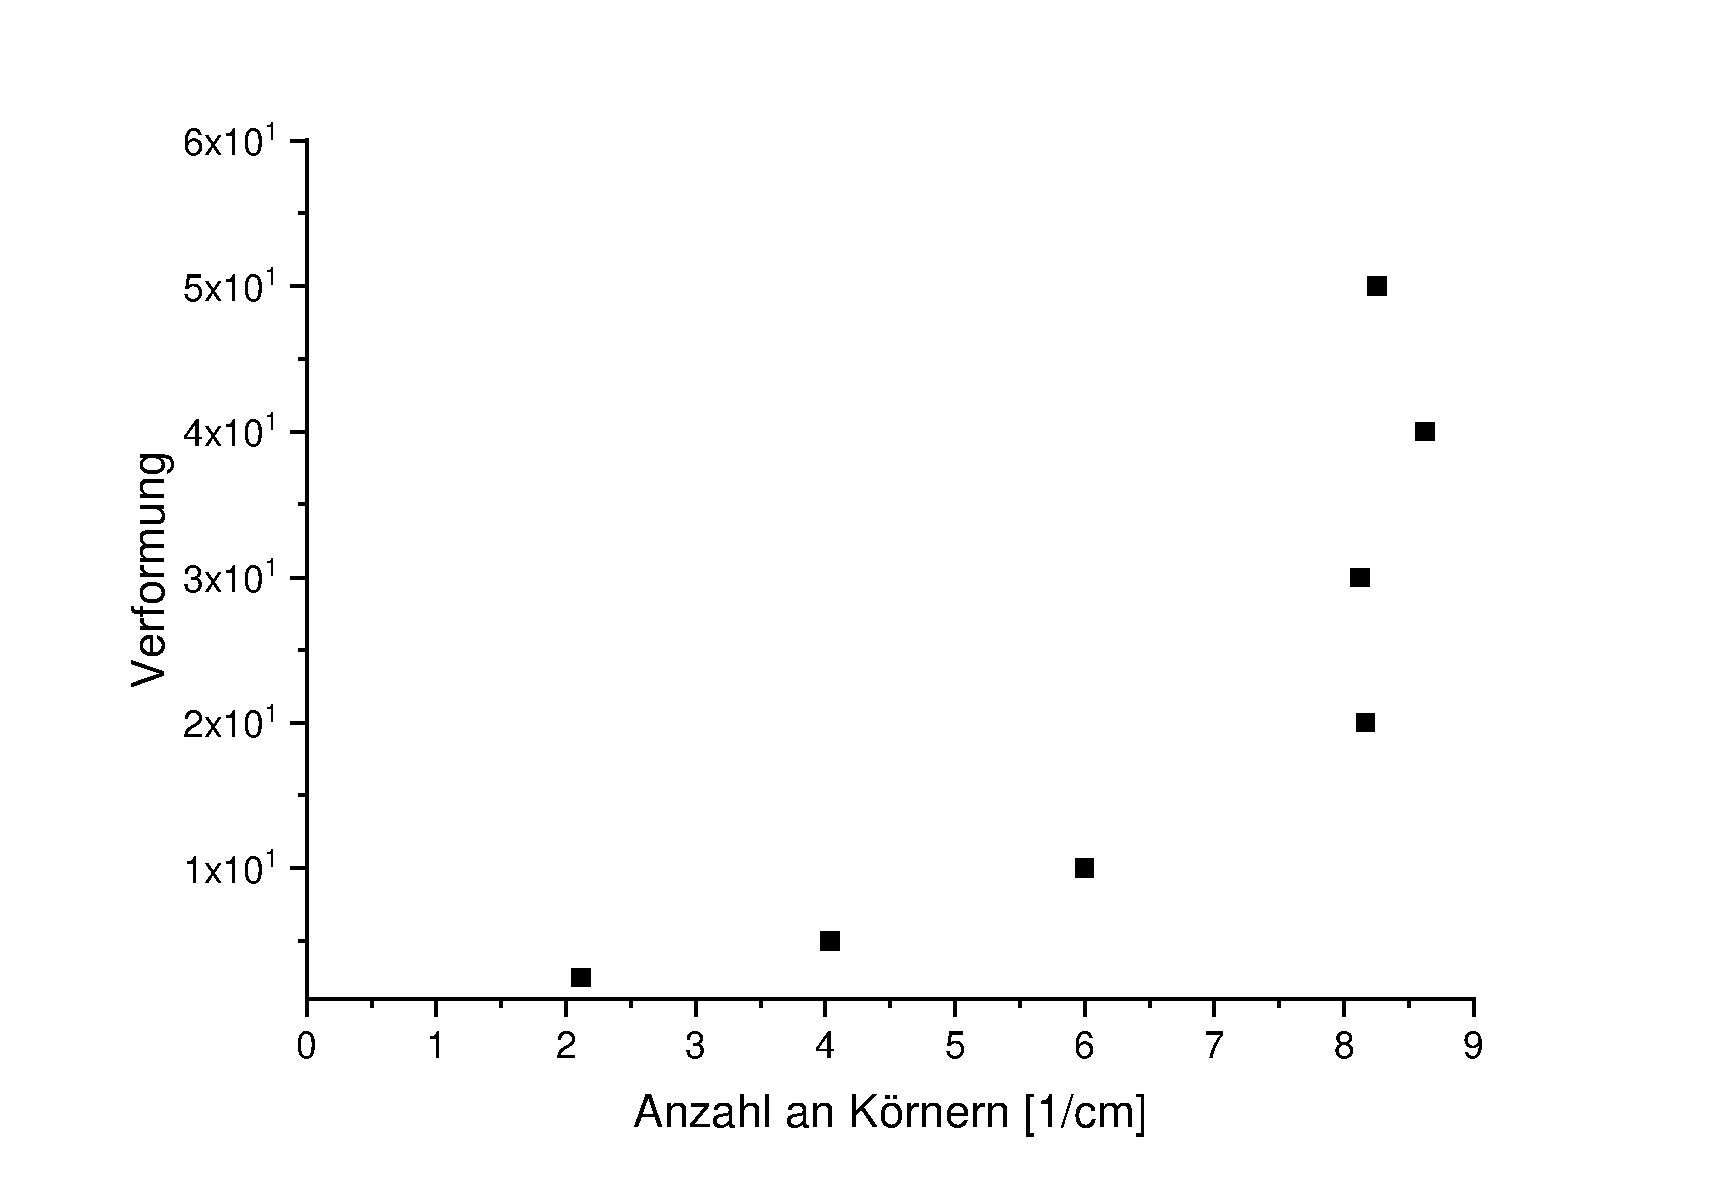
\includegraphics[scale = 0.6]{A1.pdf}
    \caption{Hier ist der Verformungsgrad in Abhängigkeit von der Anzahl an Körnern pro Zentimeter aufgetragen.}
    \label{A1}
\end{figure}
Anhand der Messwerte kann ein exponentieller Anstieg vermutet werden. Um genauer zu untersuchen, ob es sich tatsächlich um einen exponentiellen Anstieg handelt, wurden die Messwerte logarithmisch aufgetragen. Dieses Verhältnis kann in \cref{A2} berechnet werden. Die roten Punkte sind die Messwerte, an denen ein exponentieller Anstieg vermutet wird. Hierzu wird \cref{A3} einen funktionalen Zusammenhang bieten. Der blaue Punkt bei \cref{A2} stellt das Aluminiumplättchen ohne jegliche Verformung dar. Es ist zu beobachten, dass der Nullzustand eine deutlich größere Anzahl an Kristallen pro Zentimeter besitzt, als die ersten beiden Verformungszustände ($V<e^2$) . Danach erst wächst die Anzahl an Kristallen, wie bereits beschrieben, exponentiell an, bis zu einem Punkt, an dem die Messwerte konvergieren. Sie steigen nicht mehr an, sondern verteilen sich statistisch um einen Mittelwert herum.
\begin{figure}[h!]
    \centering
    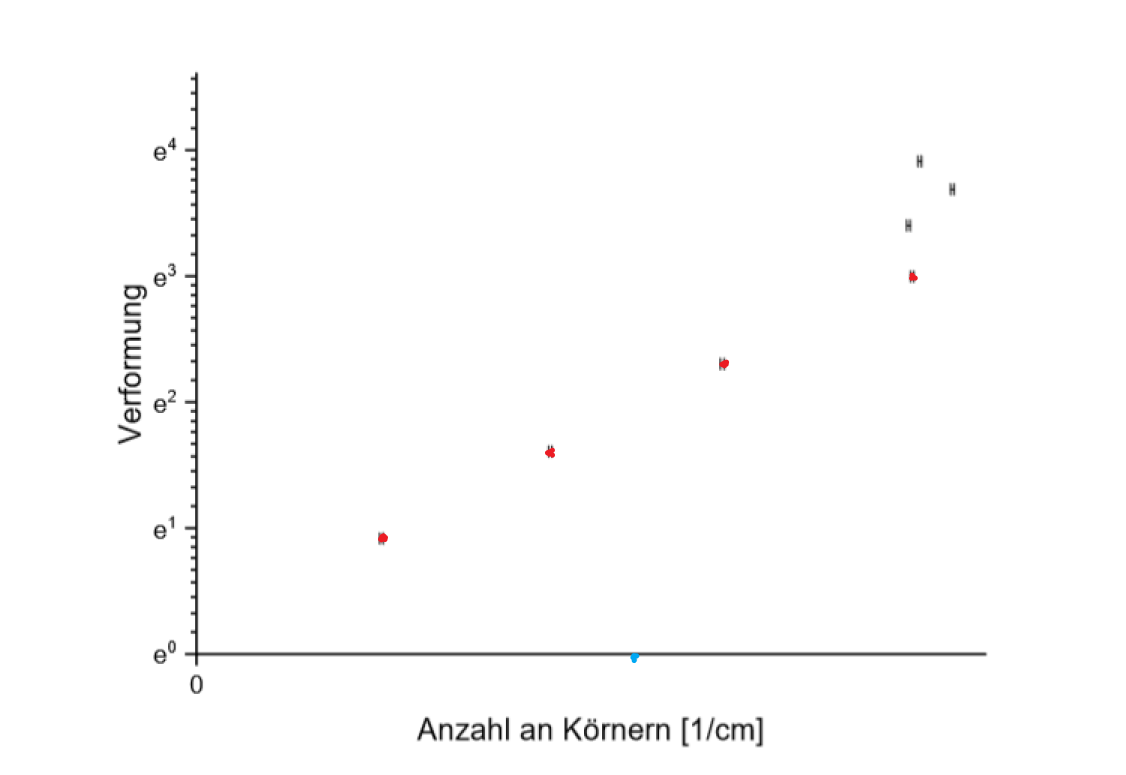
\includegraphics[scale = 0.6]{te.png}
    \caption{Der Graph stellt die Verformung in Abhängigkeit von der Anzahl der Körner dar. Die roten Punkte stellen die Messwerte da, die einen exponentiellen Zusammenhang aufweisen. Der blaue Punkt stellt den Referenzwert dar.}
    \label{A2}
\end{figure}
In \cref{A3} wurde der bereits erwähnte funktionale Zusammenhang zur Verformung und Anzahl an Kristallen dargestellt. Dieser Zusammenhang gilt nur für Verformungen bei einem Grad von etwa $e^1 - e^3$. Aufgrund des geringen Fehlers kann angenommen werden, dass in diesem Bereich tatsächlich ein exponentielles Wachstum stattfindet.
\begin{figure}[h!]
    \centering
    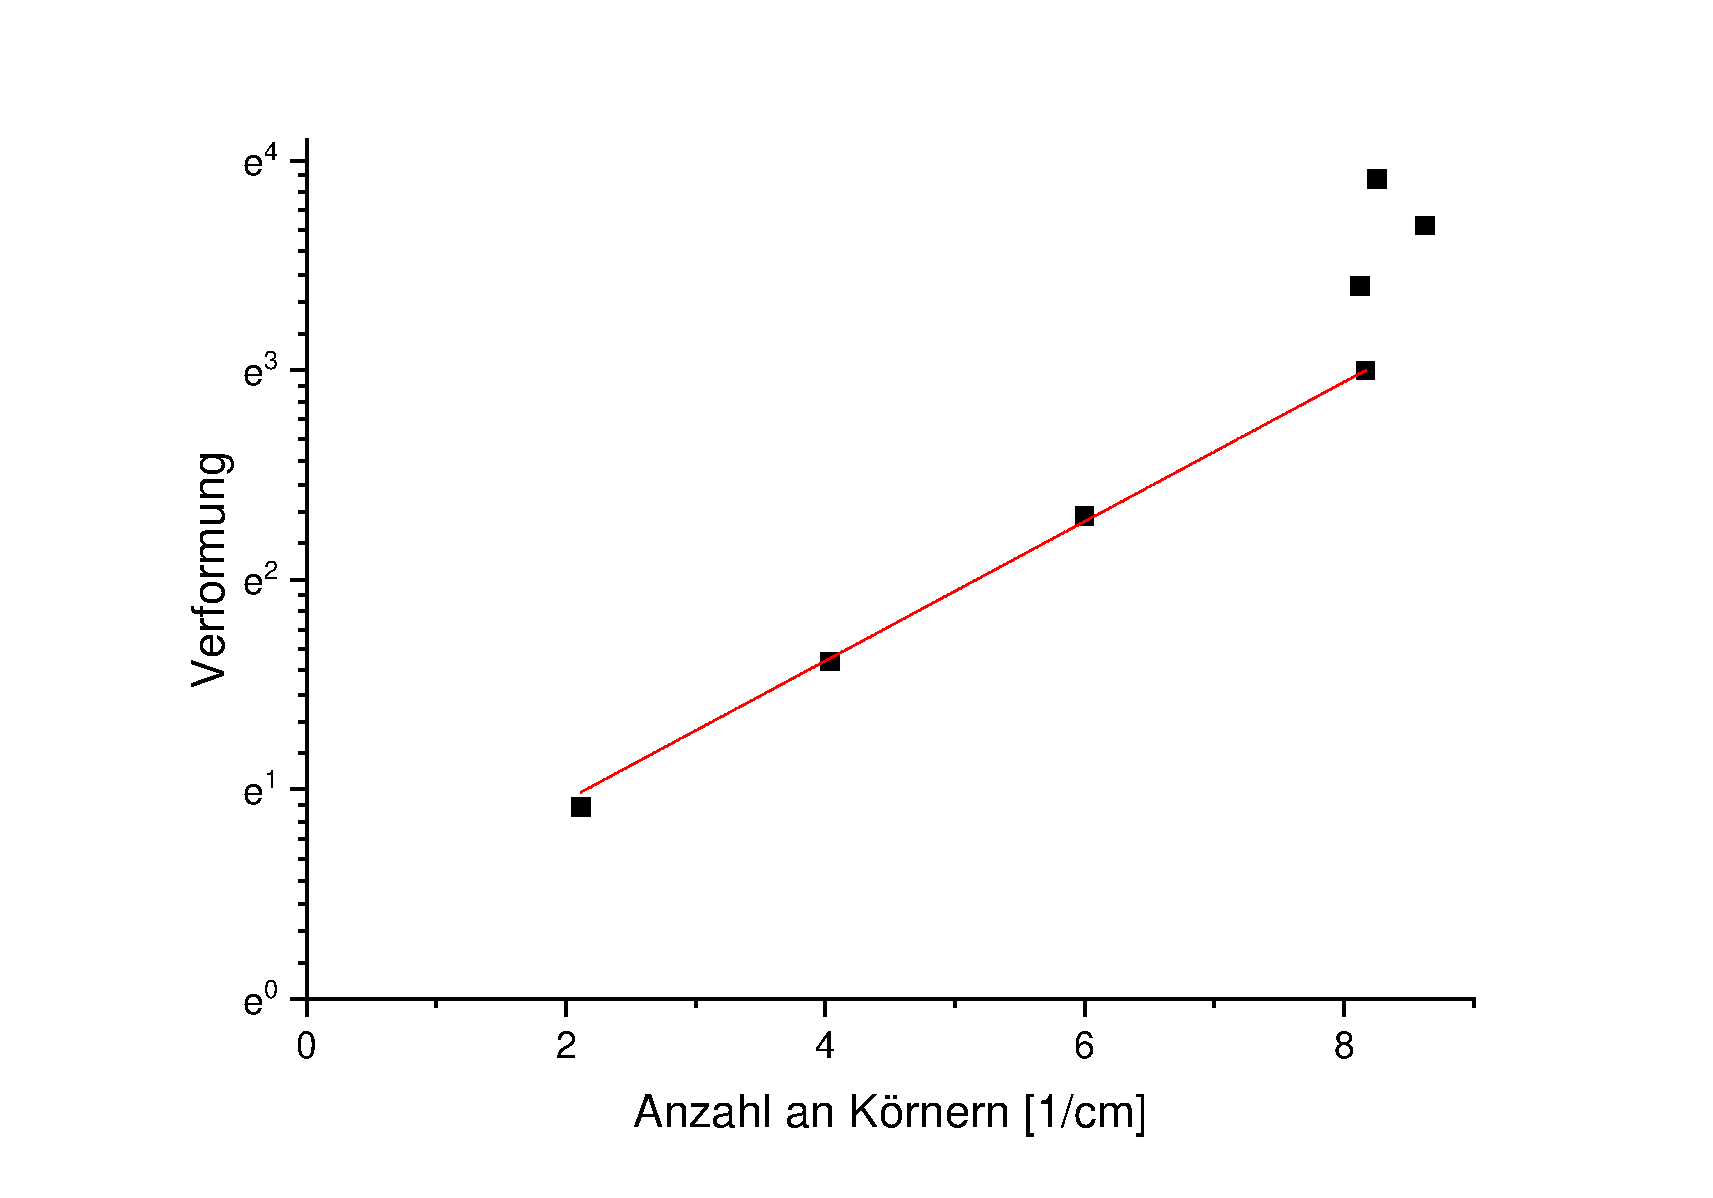
\includegraphics[scale = 0.6]{fitfit.pdf}
    \caption{Der Graph stellt die Verformung in Abhängigkeit von den Anzahl der Körner dar. Für den Fit, welcher mit Origin durchgeführt wurde, wurden nur die roten Punkte aus \cref{A2} verwendet. Die Fitparameter lauten:
    $y=ab^x$ mit Parametern $a=1,33\pm 0,08$ und $b = 1,39 \pm 0,01$.}
    \label{A3}
\end{figure}

\subsection{Unsicherheiten}
Für die Unsicherheit der Anzahl der Körner wird eine absolute Messunsicherheit von $\pm 0,1$cm für die Länge der Linie angenommen. Für das Körner zählen wird wiederum eine Unsicherheit von 5\% angenommen. Mithilfe von Fehlerfortpflanzung kann daraufhin die Unsicherheit für die Anzahl der Körner pro cm berechnet werden.

Die Unsicherheit der Verformung berechnet sich aus \cref{eq:ver}.
Da hier ein linearer Zusammenhang vorliegt, ist die Unsicherheit dieselbe wie bei d. Die Unsicherheit von der Dicke (d) wurde durch eine Dreieckswahrscheinlichkeitsdichtefunktion berechnet.
\begin{align*}
    u_d = 0,2\text{cm}
\end{align*}
Die Messunsicherheiten sind in den Graphen mitberücksichtigt worden, sind jedoch häufig so klein, dass diese nicht zu erkennen sind.


\subsection{Diskussion}
Anhand der Messwerte lässt sich einiges über das Verhalten des Stoffes herausfinden. Nur die Verformungen bei einem Grad von $e^1-e^3$ konnten beschrieben werden.\cref{A3} konnte einen exponentiellen Zuwachs von Körnern bei steigendem Verformungsgrad beobachten. Außerdem konnten noch zwei weitere Fälle beobachtet werden. Der erste Fall ist bei hohen Körnerzahlen beobachtet worden. Es scheint, als ob es eine Mindestgröße von Körnern gäbe. Wenn diese Mindestgröße erreicht ist kann ich meinen Stoff beliebig stark verformen ohne dass Körnerbildung ansetzt. Der zweite Fall ist der, dass bei der Referenzprobe (keine Verformung) mehr Körner vorhanden sind, als nach den ersten beiden Verformungsstufen, dass heißt, dass die Körnerbildung erst zurückgeht und dann wieder anwächst. dieser Zusammenhang kann ebenfalls durch mehr Messwerte im kleinen Verformungsbereich modelliert werden. Woran liegt es jedoch, dass diese beiden Fälle auftreten. Unsere Referenzprobe besitzt eine mittlere Korngröße, wenn der Stoff verformt wird, wächst die mittlere Korngröße an, jedoch besitzt der Stoff nur wenige Versetzungen, sodass sich bei dem Prozess der Rekristallisation nur wenige Körner bilden. ES werden vor allem die Körner gestreckt. Die Anzahl der Körner nimmt ab pro Zentimeter. Wenn immer stärker verformt wird, nimmt die Anzahl der Versetzungen zu und es können immer mehr Körner bei der Rekristallisation entstehen, bis zu einem Punkt, an dem so viele Versetzungen in den Kristall eingegangen sind, sodass sich die maximale Anzahl an Versetzungen bereits gebildet hat. Ab diesem Zeitpunkt würde bei größerer Verformung der Werkstoff reißen und die Anzahl an Körnen gleich bleiben, sodass hier ein Grenzwert erreicht wird.

\newpage

\begin{thebibliography}{9}
	\bibitem{A}
	Versuch zur Al-Rekristallisation,Fortgeschrittenen Praktikum, Versuchsanleitung, Münster ,WS 18/19
	
\end{thebibliography}
\end{document}
